% =====================================================================
% Paper A+B (merged) - Supplementary Information
%
% Long-form derivations supporting the main paper "Closed-form
% absorbed-power dosimetry on the human body, 1 to 100 GHz".
% Author: Robin Wydaeghe
% =====================================================================

\documentclass[journal,onecolumn,11pt]{IEEEtran}

\usepackage[utf8]{inputenc}
\usepackage[T1]{fontenc}
\usepackage{lmodern}
\usepackage{microtype}

\usepackage{amsmath,amssymb,amsthm,mathtools}
\usepackage{bm}

\usepackage{graphicx}
\graphicspath{{figures/}}
\usepackage{booktabs}
\usepackage{array}
\usepackage{caption}
\usepackage{enumitem}

\usepackage{cite}
\usepackage{xcolor}
\usepackage[colorlinks=true,linkcolor=blue,citecolor=blue,urlcolor=blue]{hyperref}
\usepackage[capitalize]{cleveref}

\theoremstyle{plain}
\newtheorem{theorem}{Theorem}[section]
\newtheorem{proposition}[theorem]{Proposition}
\newtheorem{corollary}[theorem]{Corollary}
\theoremstyle{remark}
\newtheorem{remark}[theorem]{Remark}

\renewcommand{\thesection}{S\arabic{section}}
\renewcommand{\thefigure}{S\arabic{figure}}
\renewcommand{\thetable}{S\arabic{table}}
\renewcommand{\theequation}{S\arabic{equation}}

% --- math macros ---
\newcommand{\khat}{\hat{\bm{k}}}
\newcommand{\nhat}{\hat{\bm{n}}}
\newcommand{\rr}{\mathbf{r}}
\newcommand{\EE}{\mathbf{E}}
\newcommand{\Sinc}{S_{\mathrm{inc}}}
\newcommand{\Sab}{S_{\mathrm{ab}}}
\newcommand{\Aab}{A_{\mathrm{ab}}}
\newcommand{\Aperp}{A_\perp}
\newcommand{\Teff}{T_{\mathrm{eff}}}
\newcommand{\Tavg}{T_{\mathrm{avg}}}
\newcommand{\Tbar}{\bar{T}}
\newcommand{\Tlay}{T_{\mathrm{lay}}}
\newcommand{\ntilde}{\tilde{n}}
\newcommand{\diff}{\mathrm{d}}
\newcommand{\pospart}[1]{\left[#1\right]_{+}}
\newcommand{\Vis}{V}
\DeclareMathOperator{\RE}{Re}
\DeclareMathOperator{\IM}{Im}

\begin{document}

\title{Supplementary Information for\\
``Closed-Form Absorbed-Power Dosimetry on the Human Body, 1 to 100~GHz''}

\author{Robin~Wydaeghe%
  \thanks{R. Wydaeghe is with Ghent University and imec, Ghent,
  Belgium (e-mail: robin.wydaeghe@ugent.be).}}

\maketitle

\begin{abstract}
This document presents the long-form derivations supporting the main
paper. Section~\ref{si:fresnel} derives the polarization-aware
Fresnel surface law and the three conditions under which the
polarization correction vanishes. Section~\ref{si:azzam} extends
Azzam's lossless high-index criterion to lossy biological tissue and
quantifies the resulting angular variation across the IT'IS Cole--Cole
catalog. Section~\ref{si:layered} treats the layered tissue model
behind the cube SAR below 6~GHz: Chew recursion of the generalized
Fresnel reflection coefficient, the standing-wave SAR with forward,
backward, and interference terms, layer-by-layer integration over the
10~g cube, the subsurface peak criterion, and the regimes where
the layered model itself breaks down. Section~\ref{si:mie} reports
the per-frequency Mie residual analysis on body-scale lossy spheres
with frequency-dependent IT'IS skin properties. Section~\ref{si:anthro}
gives the anthropometric scaling of the whole-body compliance
threshold. Numbering in this document is prefixed with S. Equations
and figures cited without a prefix refer to the main paper.
\end{abstract}


\section{Polarization-aware Fresnel law}\label{si:fresnel}

\subsection{Setup}
A monochromatic plane wave with time-averaged Poynting vector
$\mathbf{S}_{\mathrm{inc}} = \Sinc\,\khat$ illuminates a body whose
surface $\Sigma$ is locally flat on the wavelength scale. At a
surface point $\rr$ with outward normal $\nhat(\rr)$, the local TE
and TM unit vectors are
\begin{align}
  \hat{e}_s(\rr) &= (\khat \times \nhat) / |\khat \times \nhat|,
  \label{eq:es}\\
  \hat{e}_p(\rr) &= \hat{e}_s \times \khat\, .
  \label{eq:ep}
\end{align}
Decompose the incident electric field as
\begin{equation}\label{eq:E-decomp}
  \EE_0 = a_s\,\hat{e}_s(\rr) + a_p\,\hat{e}_p(\rr)\, ,
\end{equation}
with complex amplitudes $a_s, a_p$ that depend on the surface point
because the local TE and TM bases rotate with $\nhat(\rr)$ across
the body. The local TE and TM intensity fractions are
\begin{equation}\label{eq:e-fractions}
  |e_s(\rr)|^2 = \frac{|a_s(\rr)|^2}{|\EE_0|^2},
  \qquad
  |e_p(\rr)|^2 = \frac{|a_p(\rr)|^2}{|\EE_0|^2}\, ,
\end{equation}
and they satisfy $|e_s|^2 + |e_p|^2 = 1$ pointwise.

\subsection{Effective transmission}
The Fresnel power-transmission coefficients on a planar interface
between vacuum ($n_1 = 1$) and a lossy medium of complex refractive
index $\ntilde$ are
\begin{align}
  T_s(\theta)
  &= 1 - |r_s(\theta)|^2,
  \quad
  r_s = \frac{\mu - \xi}{\mu + \xi},
  \label{eq:Ts-SI}\\
  T_p(\theta)
  &= 1 - |r_p(\theta)|^2,
  \quad
  r_p = \frac{\ntilde^2\mu - \xi}{\ntilde^2\mu + \xi}\, ,
  \label{eq:Tp-SI}
\end{align}
with $\mu = \cos\theta_i$ and
$\xi = \sqrt{\ntilde^2 - 1 + \mu^2}$, $\RE\xi > 0$. For an incident
field of~\eqref{eq:E-decomp}, energy conservation at the interface
gives the effective transmission
\begin{equation}\label{eq:Teff-SI}
  \Teff(\rr) = |e_s(\rr)|^2\,T_s(\theta(\rr))
            + |e_p(\rr)|^2\,T_p(\theta(\rr))\, ,
\end{equation}
and the absorbed power density at a visible point is
$\Sab(\rr) = \Sinc\,\Teff(\rr)\,\pospart{\mu(\rr)}$.

\subsection{Polarization splitting}
Write
\begin{equation}\label{eq:Teff-decomp-SI}
  \Teff(\rr) = \Tavg(\theta) + \tfrac{1}{2}q(\rr)\,\Delta T(\theta)\, ,
\end{equation}
with $\Tavg = (T_s + T_p)/2$ the unpolarized baseline,
$\Delta T = T_p - T_s$ the polarization splitting, and
$q(\rr) = |e_p|^2 - |e_s|^2 \in [-1,1]$ the local TM excess. Three
conditions cancel the polarization term.

\paragraph{Circular polarization.} For circularly polarized
illumination the field's TE and TM intensities are equal at every
point on every body, $|e_s|^2 = |e_p|^2 = 1/2$ pointwise, and
$q \equiv 0$.

\paragraph{Random ensemble of linear polarizations.} For
monochromatic linearly polarized illumination with random ensemble
orientation, parameterize the polarization by an angle
$\phi \in [0, 2\pi)$ with uniform distribution. The TE and TM
projections at a point $\rr$ scale as $\cos^2\phi'$ and $\sin^2\phi'$
with $\phi'$ a body-shifted angle, and $\langle\cos^2\phi' -
\sin^2\phi'\rangle_\phi = 0$. The ensemble-averaged $\langle q \rangle$
vanishes.

\paragraph{Multipath averaging.} For a body in a multipath
environment with $N$ independent path orientations
$\{\khat_n\}_{n=1}^N$ and equal power weights, write the body
polarization directivity~\cite{Diao2024} as
\begin{equation}\label{eq:DB}
  D_B(\khat) = \frac{|\tilde{B}(\khat)|}{2|\tilde{A}_\perp(\khat)|}\, ,
\end{equation}
where $\tilde{B}$ is the off-diagonal Stokes component and
$\tilde{A}_\perp$ the diagonal projected-area component, both at the
body-integrated level. The variance of the polarization correction
to the direction-averaged absorbed power is bounded by
$D_B / \sqrt{2N}$. With $D_B = 16\%$ on the Thelonious phantom and
$N = 20$ paths, the correction is below $2.5\%$.

Under any of these three conditions, $\Teff \to \Tavg(\theta)$, and
the local law reduces to $\Sab(\rr) = \Sinc\,\Tavg(\theta(\rr))\,
\pospart{\mu(\rr)}$.


\section{Pseudo-Brewster compensation across tissues}\label{si:azzam}

\subsection{Azzam's high-index criterion}
Azzam~\cite{Azzam2015} showed that for a lossless dielectric
substrate with refractive index $|\ntilde| > 2 + \sqrt{3} \approx
3.73$, the unpolarized reflectance varies by less than $1\%$ over
$[0^\circ, 60^\circ]$. The criterion follows from a series expansion
of $|r_s|^2 + |r_p|^2$ around the pseudo-Brewster angle
$\theta_{pB} = \arctan|\ntilde|$. The leading angular dependence
cancels at $|\ntilde|^2 = 2 + \sqrt{3}$, leaving a quartic residual.

The criterion weakens for $|\ntilde| > 2.5$, where the unpolarized
reflectance varies by less than $6\%$ over $[0^\circ, 75^\circ]$.
We extend the criterion empirically to lossy biological tissue
$\ntilde = n - i\kappa$ and verify on the IT'IS catalog.

\subsection{Quantitative evaluation across IT'IS tissues}
\Cref{tab:itis-pB} reports $\ntilde$, $T_0$, and the maximum angular
variation of $\Tavg/T_0$ on the IT'IS v5.0 catalog across 0.3
to 100~GHz. For every tissue with $|\ntilde| > 2.5$, the variation
stays below $6\%$ over $[0^\circ, 60^\circ]$ and within a few percent
over $[0^\circ, 75^\circ]$. \Cref{fig:si-tissue-universality} shows
this directly. High-index tissues (skin, muscle, brain, eye) form a
near-flat plateau through wide angles. Fat has $|\ntilde| \approx
2.05$ at 28~GHz and is the only catalog entry that drops below
the band before $60^\circ$. Fat is rarely the outermost tissue at
exposure sites of regulatory interest.

\begin{figure}[!t]
  \centering
  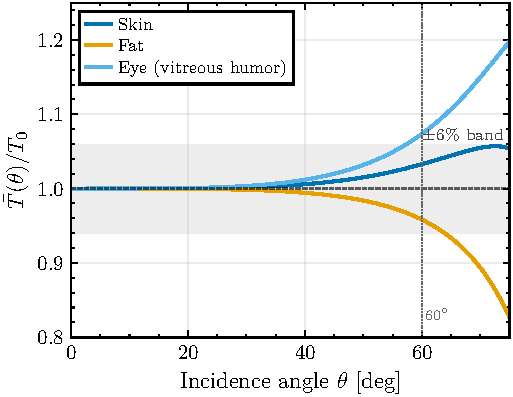
\includegraphics[width=0.78\columnwidth]{si_tissue_universality.pdf}
  \caption{Pseudo-Brewster compensation across the IT'IS v5.0
  catalog at 28~GHz: $\Tavg(\theta)/T_0$ for six representative
  tissues spanning $|\ntilde| \in [2.05, 7.19]$. The shaded band
  marks $\pm 6\%$. High-index tissues stay within a few percent
  through $60^\circ$ and bend upward only near grazing, where the
  TM channel approaches its pseudo-Brewster minimum. Fat, with
  $|\ntilde|$ below the Azzam threshold of $2.5$, is the sole
  catalog outlier dropping out of the band.}
  \label{fig:si-tissue-universality}
\end{figure}

\begin{table}[!t]
\centering
\caption{Pseudo-Brewster compensation on the IT'IS v5.0 catalog
at 28~GHz. The variation column is the maximum deviation of
$\Tavg/T_0$ from unity over $[0^\circ, 75^\circ]$.}
\label{tab:itis-pB}
\begin{tabular}{lcccccc}
\toprule
Tissue & $\varepsilon_r$ & $\sigma$ [S/m] & $|\ntilde|$ & $T_0$
  & $\theta_{pB}$ & $\Tavg$ var. \\
\midrule
Skin            & 17.0 & 25.0 & 4.84 & 0.54 & $78^\circ$ & $5.6\%$ \\
Muscle          & 25.0 & 30.0 & 5.62 & 0.48 & $80^\circ$ & $4.8\%$ \\
Brain (white)   & 12.0 & 18.0 & 4.07 & 0.59 & $76^\circ$ & $6.2\%$ \\
Brain (gray)    & 18.5 & 25.0 & 4.92 & 0.53 & $78^\circ$ & $5.5\%$ \\
Fat             &  4.0 &  2.0 & 2.05 & 0.77 & $64^\circ$ & $8.2\%$ \\
Bone (cortical) &  6.5 &  5.0 & 2.84 & 0.69 & $71^\circ$ & $7.0\%$ \\
Eye (cornea)    & 28.0 & 38.0 & 6.06 & 0.45 & $81^\circ$ & $4.4\%$ \\
Eye (vitreous)  & 39.0 & 53.0 & 7.06 & 0.40 & $82^\circ$ & $3.8\%$ \\
Water           & 25.0 & 55.0 & 6.62 & 0.45 & $81^\circ$ & $3.9\%$ \\
\bottomrule
\end{tabular}
\end{table}

\subsection{Frequency window of validity}
Across 0.3--100~GHz, the IT'IS Cole--Cole tail keeps skin
$|\ntilde|$ above $3$ (\cref{tab:itis-fvs}). The pseudo-Brewster
crossover where $T_0/\Tbar = 1$ is at 40.4~GHz. Below this
frequency $T_0$ underestimates the flux-weighted absorbed power
(conservative for compliance). Above, it overestimates by at most
$3.5\%$ at 100~GHz. The root-mean-square error stays below
$5\%$ across the band. \Cref{fig:si-angle-family} shows the angular
profile $\Tavg(\theta)\cos\theta$ at six representative frequencies.
The family is nearly indistinguishable from the simplified
$T_0\cos\theta$ across the wireless band.

\begin{figure}[!t]
  \centering
  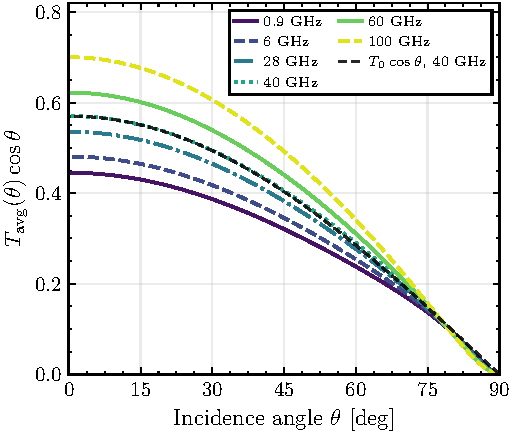
\includegraphics[width=\columnwidth]{R_of_f_angle_family.pdf}
  \caption{Pseudo-Brewster compensation across the wireless band on
  skin: $\Tavg(\theta)\cos\theta$ at six frequencies from 0.9 to
  100~GHz, with the simplified $T_0\cos\theta$ prediction at
  40~GHz overlaid (dashed). The collapse to a near-universal
  geometric profile is the visual content of the pseudo-Brewster
  compensation across the band.}
  \label{fig:si-angle-family}
\end{figure}

\begin{table}[!t]
\centering
\caption{Frequency-resolved Cole--Cole values for skin (IT'IS v5.0)
showing $T_0$, $\Tbar$, $R = T_0/\Tbar$, and the skin depth.}
\label{tab:itis-fvs}
\begin{tabular}{rccccc}
\toprule
$f$\,[GHz] & $\varepsilon_r$ & $\sigma$ [S/m] & $|\ntilde|$
  & $T_0$ & $R = T_0/\Tbar$ \\
\midrule
0.3  & 60.0 & 0.40 & 7.93 & 0.381 & 0.938 \\
0.9  & 41.4 & 0.87 & 6.70 & 0.445 & 0.957 \\
2.4  & 38.0 & 1.46 & 6.29 & 0.470 & 0.964 \\
6.0  & 35.6 & 4.00 & 6.07 & 0.481 & 0.968 \\
10   & 31.3 & 8.01 & 5.87 & 0.489 & 0.971 \\
28   & 16.6 & 25.8 & 4.84 & 0.536 & 0.988 \\
40   & 11.6 & 30.0 & 4.30 & 0.570 & 1.000 \\
60   &  7.98 & 36.4 & 3.68 & 0.622 & 1.015 \\
100  &  6.35 & 50.0 & 3.01 & 0.701 & 1.035 \\
\bottomrule
\end{tabular}
\end{table}


\section{Layered tissue model and the cube SAR}\label{si:layered}

\subsection{Frequency transition}
Three dimensionless parameters govern the transition between the
thin-skin and the layered cube SAR regimes. The depth parameter
$2\alpha L$ compares the SAR penetration depth to the cube side
$L = 21.5$~mm. The depth efficiency $h(2\alpha L)$ is the fraction
of the surface SAR surviving mass-averaging to depth $L$. The
capture fraction $C = 1 - e^{-2\alpha L}$ is the fraction of
transmitted power absorbed within the cube depth.
At 28~GHz, $2\alpha L \approx 47$ for skin and $C \approx 1$: the
thin-skin shortcut applies. At 2.45~GHz, $2\alpha L \approx 1.9$
and $C \approx 0.85$, with $15\%$ of transmitted power passing
through the cube into deeper tissue. Below 1~GHz, $2\alpha L$
falls to order unity and the homogeneous half-space breaks down
because the field passes through multiple tissue layers within the cube.

\subsection{Three-layer model and Chew recursion}
A three-layer planar model is used:
skin (epidermis + dermis, $d_1 \approx 2$~mm), subcutaneous fat
($d_2 \approx 5$--20~mm), semi-infinite muscle. At 2.45~GHz
the three layers carry contrasting dielectric properties:

\begin{table}[!t]
\centering
\caption{Tissue properties at 2.45~GHz from the IT'IS
catalog~\cite{ITISv5,Gabriel1996}.}
\label{tab:layers-2g45}
\begin{tabular}{lccccc}
\toprule
Tissue & $\varepsilon_r$ & $\sigma$ [S/m] & $n$ & $\kappa$
  & $\delta_{\mathrm{SAR}}$\,[mm] \\
\midrule
Skin   & 38.0 & 1.46 & 6.22 & 0.860 & 11.3 \\
Fat    &  5.3 & 0.08 & 2.31 & 0.127 & 76.5 \\
Muscle & 52.7 & 1.74 & 7.31 & 0.873 & 11.2 \\
\bottomrule
\end{tabular}
\end{table}

Fat is nearly transparent
($\delta_{\mathrm{SAR}} = 76.5$~mm), while skin and muscle are
lossy. The wave passes through a thick fat layer with little
attenuation and reaches the fat-muscle interface, where the
impedance mismatch produces a strong backward wave with reflection
$|r_{2,3}| \approx 0.52$.

Define the normal-incidence Fresnel coefficient at the interface
between layers $j$ and $j+1$,
\begin{equation}\label{eq:rjj1-SI}
  r_{j,j+1} = \frac{\ntilde_j - \ntilde_{j+1}}{\ntilde_j + \ntilde_{j+1}}\, ,
\end{equation}
and the one-way propagation factor across layer $j$,
\begin{equation}\label{eq:Pj-SI}
  P_j = e^{-i k_0 \ntilde_j d_j} = e^{-\alpha_j d_j}\,e^{-i\beta_j d_j}\, ,
\end{equation}
with $\alpha_j = k_0\kappa_j$ and $\beta_j = k_0 n_j$. The
generalized reflection coefficient at each interface follows the
Chew recursion~\cite{Chew1995},
\begin{align}
  \widetilde\Gamma_3 &= r_{2,3},\label{eq:Gamma3-SI}\\
  \widetilde\Gamma_2 &= \frac{r_{1,2}
    + \widetilde\Gamma_3\,P_2^{2}}
    {1 + r_{1,2}\,\widetilde\Gamma_3\,P_2^{2}},
    \label{eq:Gamma2-SI}\\
  \widetilde\Gamma_1 &= \frac{r_{0,1}
    + \widetilde\Gamma_2\,P_1^{2}}
    {1 + r_{0,1}\,\widetilde\Gamma_2\,P_1^{2}}\, ,
    \label{eq:Gamma1-SI}
\end{align}
with $r_{0,1} = (1 - \ntilde_1)/(1 + \ntilde_1)$. The overall power
transmission coefficient replacing $T_0$ in the cube SAR is
\begin{equation}\label{eq:T-layered-SI}
  \Tlay = 1 - |\widetilde\Gamma_1|^2\, .
\end{equation}

\Cref{fig:si-tlay-fr} shows $\Tlay(f)$ across 0.3--10~GHz for
the canonical 2~mm skin / 10~mm fat / muscle stack against the
skin-only baseline $T_0(f)$. The layered transmission departs
strongly from the half-space prediction in this regime. A
fat-transparent peak near 1.3~GHz appears where the 10~mm fat
layer is electrically thin and the air-skin interface is the only
significant reflector. A deep dip near 3.3~GHz appears where the
fat layer is approximately a quarter-wave thick and the round-trip
phase through fat flips the impedance seen at the air-skin interface
back into a strong mismatch. The half-space $T_0$ curve, by
construction, reproduces none of this structure. The departure motivates the
layer-resolved Chew formulation throughout this section.

\begin{figure}[!t]
  \centering
  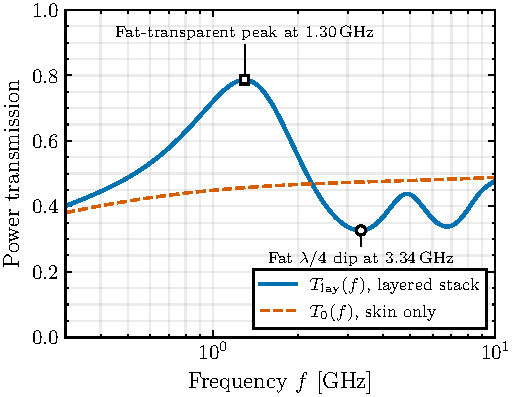
\includegraphics[width=0.78\columnwidth]{si_tlay_fat_resonance.pdf}
  \caption{Layered power transmission $\Tlay(f)$ at normal incidence
  for the 2~mm skin / 10~mm fat / semi-infinite muscle stack,
  IT'IS v5.0 Cole--Cole properties, with the skin-only $T_0(f)$
  baseline overlaid. The fat layer's electrical thickness sweeps
  through quarter-wave and half-wave conditions across the band,
  producing a transparent peak near 1.3~GHz and a $\lambda/4$ dip
  near 3.3~GHz that the homogeneous half-space model misses
  entirely.}
  \label{fig:si-tlay-fr}
\end{figure}

\subsection{Standing-wave SAR}
Inside layer $j$, with $z$ measured from the top of that layer, the
electric field has the form
\begin{equation}\label{eq:Ej-SI}
  E_j(z) = A_j\bigl[e^{-i k_j z} + g_j\,e^{+i k_j z}\bigr],
  \quad
  k_j = k_0\ntilde_j\, ,
\end{equation}
with $g_j = \widetilde\Gamma_{j+1}\,P_j^{2}$ the
backward-to-forward amplitude ratio at the top of the layer
($g_3 = 0$ for the semi-infinite muscle). The amplitudes are linked
by continuity of the tangential field at each interface,
\begin{equation}\label{eq:A-recursion}
  A_{j+1}(1 + g_{j+1})
  = A_j\,e^{-i k_j d_j}\bigl[1 + g_j\,e^{2i k_j d_j}\bigr]\, ,
\end{equation}
and $A_1$ follows from the incident amplitude through the air-skin
transmission $1 - |\widetilde\Gamma_1|^2$.

The squared modulus expands into three terms,
\begin{equation}\label{eq:E2-three-SI}
  \bigl|e^{-i k_j z} + g_j e^{i k_j z}\bigr|^2
  = e^{-2\alpha_j z} + |g_j|^2 e^{+2\alpha_j z}
  + 2|g_j|\cos(2\beta_j z + \psi_j)\, ,
\end{equation}
with $\psi_j = \arg g_j$. The SAR in layer $j$ is therefore
\begin{equation}\label{eq:SAR-standing-SI}
  \mathrm{SAR}_j(z) = \frac{\sigma_j |A_j|^2}{2\rho_j}\!
  \left[e^{-2\alpha_j z} + |g_j|^2 e^{+2\alpha_j z}
  + 2|g_j|\cos(2\beta_j z + \psi_j)\right]\, .
\end{equation}
The three terms are forward decay, backward growth, and the
coherent interference between them. The half-space limit recovers
when $g_j = 0$.

\Cref{fig:si-sar-z} renders~\eqref{eq:SAR-standing-SI} for the
canonical 2~mm skin / 10~mm fat / muscle stack at 2.45~GHz
under unit-intensity normal incidence. The SAR stays high in the
lossy skin layer because the high conductivity absorbs the incident
flux quickly. It then drops several orders of magnitude in the
low-loss fat, then rises again as the wave couples into muscle.
The subsurface peak at $z \approx 1.6$~mm is inside skin, in
agreement with the criterion of \cref{eq:subsurface-criterion-SI}
below.

\begin{figure}[!t]
  \centering
  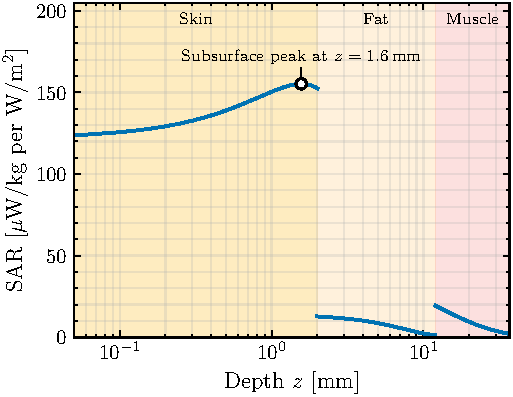
\includegraphics[width=\columnwidth]{si_standing_wave_sar.pdf}
  \caption{Standing-wave SAR profile $\mathrm{SAR}(z)$ across
  2~mm skin / 10~mm fat / semi-infinite muscle at
  2.45~GHz, normal incidence, IT'IS v5.0 properties. The
  shaded bands mark the three layers. The subsurface peak (open
  circle) is set by the standing-wave
  structure of~\eqref{eq:SAR-standing-SI}. For this stack it falls inside the
  skin layer.}
  \label{fig:si-sar-z}
\end{figure}

\subsection{Cube integral}
The integral of $\mathrm{SAR}_j\,\rho_j$ over the full thickness of
a finite layer $j$ admits a closed form,
\begin{multline}\label{eq:layer-integral-SI}
  \int_0^{d_j}\mathrm{SAR}_j\,\rho_j\,\diff z
  = \frac{\sigma_j |A_j|^2}{2}\biggl[
    \frac{1 - e^{-2\alpha_j d_j}}{2\alpha_j}
  + |g_j|^2\,\frac{e^{2\alpha_j d_j} - 1}{2\alpha_j}\\
  + \frac{|g_j|}{\beta_j}\bigl(\sin(2\beta_j d_j + \psi_j)
    - \sin\psi_j\bigr)
  \biggr]\, .
\end{multline}
For the semi-infinite muscle ($g_3 = 0$, depth $d_3 = L - d_1 -
d_2$) only the forward term survives,
\begin{equation}\label{eq:muscle-integral-SI}
  \int_0^{d_3}\mathrm{SAR}_3\,\rho_3\,\diff z
  = \frac{\sigma_3 |A_3|^2}{2}\,
  \frac{1 - e^{-2\alpha_3 d_3}}{2\alpha_3}\, .
\end{equation}
The peak spatial-average SAR over the cube is the sum of the layer
contributions divided by the total tissue mass,
\begin{equation}\label{eq:psSAR-layered-SI}
  \langle\mathrm{SAR}\rangle_{\mathrm{cube}}
  = \frac{1}{m}\sum_{j=1}^{3}\int_0^{\min(d_j, z_j^{\max})}
    \mathrm{SAR}_j\,\rho_j\,\diff z\, .
\end{equation}

\subsection{Subsurface peak criterion}
In the homogeneous half-space, the SAR maximum is at $z = 0$
because $e^{-2\alpha z}$ is monotonic. Differentiating
\eqref{eq:SAR-standing-SI} in skin (layer 1) at the surface,
\begin{equation}\label{eq:dSAR-dz-SI}
  \frac{\diff\mathrm{SAR}_1}{\diff z}\bigg|_{z=0}
  = \frac{\sigma_1 |A_1|^2}{2\rho_1}
  \bigl[-2\alpha_1 + 2\alpha_1|g_1|^2 - 4\beta_1|g_1|\sin\psi_1\bigr]\, .
\end{equation}
Dividing by $2\alpha_1 > 0$ gives the criterion for a subsurface
SAR maximum,
\begin{equation}\label{eq:subsurface-criterion-SI}
  |g_1|^2 - \frac{2\beta_1}{\alpha_1}\,|g_1|\sin\psi_1 > 1\, .
\end{equation}
The criterion has two contributions. The reflection-strength term
$|g_1|^2$ rarely exceeds unity on its own. Typical values at
2.45~GHz are $|g_1| \approx 0.6$, giving $|g_1|^2 \approx 0.37$.
The interference term $-(2\beta_1/\alpha_1)|g_1|\sin\psi_1$
dominates because $\beta_1/\alpha_1 = n_1/\kappa_1 \approx 7$ for
skin at 2.45~GHz, and even modest reflections $|g_1| \approx 0.6$
with negative $\psi_1$ produce a large positive contribution.

For a 2~mm skin / 10~mm fat / muscle stack at 2.45~GHz,
$|g_1| = 0.61$, $\psi_1 = -61^\circ$, and the criterion evaluates
to $0.37 + 7.7 = 8.0 \gg 1$. Thin lossy skin over thick low-loss
fat over lossy muscle gives a Fabry--P\'erot enhancement of order
$[(1+|g_1|)/(1-|g_1|)]^2$ at standing-wave antinodes, factors of
$2$--$4$ for typical anatomy.

\subsection{Where the layered model breaks}
Three phenomena invalidate the layered planar half-space at
sufficiently low frequencies.

\paragraph{Whole-body resonance, below approx.\ 300~MHz.}
When the free-space wavelength becomes comparable to body height
($\lambda/2 \approx 0.85$~m at approximately 175~MHz, with the resonance
peaked near 70~MHz for a grounded standing
adult~\cite{Durney1986}), the human body acts as a resonant dipole
antenna. Internal fields are dominated by whole-body current
distributions, not by the surface-transmitted plane wave. Localized
hotspots form at anatomical constrictions (ankles, wrists, neck)
where current density is highest. These hotspot locations bear no
relation to the surface absorbed power density. The
surface-to-volume reduction does not apply.

\paragraph{Finite-thickness anatomy.}
Thin features such as the ear pinna (cartilage thickness
approximately 2~mm) violate the semi-infinite half-space assumption even
at higher frequencies. At 2~GHz, $\alpha d \approx 0.09$ for a
2~mm ear, so the one-way attenuation is only $0.91$. The
transmitted field partially exits the far side and illuminates the
opposite surface. The SAR in such structures requires a
finite-slab transmission model rather than a half-space model.

\paragraph{Body-traversing multipath.}
At frequencies where $\delta_{\mathrm{SAR}}$ exceeds the body
diameter at narrow cross-sections (e.g., $\delta_{\mathrm{SAR}}
\approx 20$~mm at 900~MHz versus forearm diameter
approximately 60~mm), the field transmitted through one side reaches the
opposite side. Reflections from the far body-air interface create a
second backward wave, and the resulting interference pattern can
produce deep hotspots at locations not predictable from the surface
fields alone.


\section{Mie residual analysis}\label{si:mie}

For a lossy sphere of radius $a$ and complex refractive index
$\ntilde$, the Mie series gives an exact absorption efficiency
$Q_{\mathrm{abs}}(x, \ntilde)$ where $x = \pi d/\lambda$ is the size
parameter. The geometric law predicts $Q^{\mathrm{geom}} = T_0$, and
the relative error is $(T_0/Q_{\mathrm{abs}} - 1)\times 100\%$.

The error decomposes as
\begin{equation}\label{eq:mie-error-decomp}
  \frac{T_0}{Q_{\mathrm{abs}}} - 1
  = \underbrace{\bigl(T_0/\langle\Tavg\rangle_{\mathrm{sphere}}
    - 1\bigr)}_{\mathrm{Fresnel}}
    + \underbrace{\bigl(\langle\Tavg\rangle_{\mathrm{sphere}}
    /Q_{\mathrm{abs}} - 1\bigr)}_{\mathrm{diffraction}}\, ,
\end{equation}
with the Fresnel term shape- and frequency-dependent but
size-independent (the sphere ratio $R_{\mathrm{sphere}}(f) =
T_0/\langle\Tavg\rangle$ that crosses unity at approximately 39~GHz on
skin), and the diffraction term scaling as $x^{-2/3}$ in the optical
regime, with the wave bending into the geometric shadow and adding
absorption that the surface law misses.

\Cref{tab:mie-residual} reports the residual at six frequencies on
four representative body-part diameters with frequency-dependent
IT'IS skin properties. The mmWave band stays within 5--14\%
on body-relevant sizes (head, torso). Fingers below 6~GHz are
the worst case, with errors above $30\%$. On body-scale objects in
the claimed regime, the residual is comparable to the $\pm 7\%$
envelope on $T_0$ that follows from the $\pm 20\%$ input
uncertainty on the IT'IS dielectric properties.

\begin{table}[!t]
\centering
\caption{Mie residual $T_0/Q_{\mathrm{abs}} - 1$ in percent on
lossy spheres with frequency-dependent IT'IS skin properties.
Negative values mean the surface law underestimates absorption.}
\label{tab:mie-residual}
\begin{tabular}{rcccc}
\toprule
$f$\,[GHz] & Finger (17~mm) & Arm (80~mm)
  & Head (180~mm) & Torso (300~mm) \\
\midrule
1   & $-58$ & $-44$ & $-32$ & $-23$ \\
3   & $-42$ & $-25$ & $-15$ & $-9.4$ \\
6   & $-32$ & $-15$ & $-7.6$ & $-4.8$ \\
10  & $-24$ & $-9.0$ & $-4.5$ & $-2.7$ \\
28  & $-12$ & $-3.8$ & $-1.9$ & $-1.4$ \\
60  & $-5.2$ & $-1.8$ & $-1.4$ & $-1.3$ \\
100 & $-2.6$ & $-1.0$ & $-1.0$ & $-1.0$ \\
\bottomrule
\end{tabular}
\end{table}


\section{Anthropometric scaling}\label{si:anthro}

The whole-body compliance threshold from the main paper is
\begin{equation}\label{eq:Sinc-max-SI}
  \Sinc^{\max} = \frac{0.16\,m}{\Tbar\,\Aab}\, ,
\end{equation}
with $\Aab = \bar\eta\,A$ where $A$ is the body surface area and
$\bar\eta = \Aab/A$ the area-weighted exposure fraction.

\subsection{Du Bois scaling of body surface area}
The empirical Du Bois formula~\cite{DuBois1916} gives
\begin{equation}\label{eq:du-bois}
  A = 0.007184\,m^{0.425}\,h^{0.725}\, ,
\end{equation}
in m$^2$ with mass $m$ in kg and height $h$ in cm. The threshold
scales as $m/A$, so
\begin{equation}\label{eq:Sinc-anthro}
  \Sinc^{\max} \propto \frac{m}{A}
  \propto m^{0.575}\,h^{-0.725}
  = \mathrm{BMI}^{0.575}\,h^{0.425}\, ,
\end{equation}
recovering the dosimetry-literature observation~\cite{Hirata2007corr,
Dimbylow2002} that absorption cross-section scales with surface area
while mass scales with volume.

\subsection{Population evaluation}
\Cref{tab:anthro-SI} evaluates~\eqref{eq:Sinc-max-SI} on a
representative population at 28~GHz with $T_0 = 0.536$ and
$\bar\eta = 0.85$. The threshold varies by a factor of approximately
two between an infant and a large adult.

\begin{table}[!t]
\centering
\caption{Compliance threshold across body sizes at 28~GHz with
$T_0 = 0.536$ and $\bar\eta = 0.85$.}
\label{tab:anthro-SI}
\begin{tabular}{lccccc}
\toprule
Body type & $m$ [kg] & $h$ [cm] & $A$ [m$^2$]
  & $m/A$ [kg/m$^2$] & $\Sinc^{\max}$ [W/m$^2$] \\
\midrule
Infant (1~yr)    &   8 &  70 & 0.379 & 21.1 &  6.2 \\
Child (6~yr)     &  20 & 110 & 0.776 & 25.8 &  7.6 \\
Adolescent       &  50 & 160 & 1.491 & 33.5 &  9.9 \\
Adult (ref.)     &  70 & 170 & 1.810 & 38.7 & 11.4 \\
Large adult      & 100 & 180 & 2.193 & 45.6 & 13.5 \\
\bottomrule
\end{tabular}
\end{table}

The reference adult clears the ICNIRP general-public reference
level of 10~W/m$^2$ at 28~GHz under worst-case directional
exposure, while smaller body sizes carry lower thresholds.

\subsection{Polarization worst case}
Linearly polarized illumination at the most sensitive direction
shifts $\Tbar$ in~\eqref{eq:Sinc-max-SI} by at most a fraction
$|\tilde{B}|/(2\tilde A_\perp) \le D_B$, with $D_B = 16\%$ on the
Thelonious anatomical phantom and $D_B \le 27.9\%$ on the
worst-case convex shape (an infinite cylinder at broadside). For
multipath environments with $N \ge 20$ independent path
orientations, the correction is below $2.5\%$ via the
$D_B/\sqrt{2N}$ scaling of \cref{si:fresnel}. The unpolarized
\eqref{eq:Sinc-max-SI} is therefore conservative for any
reverberation chamber and for the most common exposure scenario, a
vertically polarized base-station illumination of a standing
person.


\begin{thebibliography}{10}
\providecommand{\url}[1]{#1}

\bibitem{Diao2024}
Y.~Diao, S.~Kodera, K.~Li, and A.~Hirata, ``Assessment of
  whole-body-average SAR for exposure to electromagnetic fields up to
  30~GHz using a body model with scaled dielectric parameters,''
  \emph{IEEE Trans. Electromagn. Compat.}, vol.~66, no.~5,
  pp.~1351--1360, Oct. 2024.

\bibitem{Azzam2015}
R.~M.~A. Azzam, ``High-index dielectric substrates with nearly constant
  reflectance for incident unpolarized or circularly polarized light over
  a wide range of incidence angles,'' \emph{J. Mod. Opt.}, vol.~62,
  no.~10, pp.~811--815, Jun. 2015.

\bibitem{ITISv5}
IT'IS Foundation, ``Tissue properties database V5.0,'' Z\"urich,
  Switzerland, 2024. [Online]. Available:
  \url{https://itis.swiss/virtual-population/tissue-properties/database/}

\bibitem{Gabriel1996}
S.~Gabriel, R.~W. Lau, and C.~Gabriel, ``The dielectric properties of
  biological tissues: III. Parametric models for the dielectric spectrum
  of tissues,'' \emph{Phys. Med. Biol.}, vol.~41, no.~11,
  pp.~2271--2293, Nov. 1996.

\bibitem{Chew1995}
W.~C. Chew, \emph{Waves and Fields in Inhomogeneous Media}.\quad
  New York, NY, USA: IEEE Press, 1995.

\bibitem{Durney1986}
C.~H. Durney, H.~Massoudi, and M.~F. Iskander, \emph{Radiofrequency
  Radiation Dosimetry Handbook}, 4th~ed.\quad Brooks Air Force Base,
  TX, USA: USAFSAM, 1986, USAFSAM-TR-85-73.

\bibitem{DuBois1916}
D.~Du~Bois and E.~F. Du~Bois, ``Clinical calorimetry: Tenth paper.
  A formula to estimate the approximate surface area if height and
  weight be known,'' \emph{Arch. Intern. Med.}, vol.~17, no.~6,
  pp.~863--871, Jun. 1916.

\bibitem{Hirata2007corr}
A.~Hirata, Y.~Nagaya, O.~Fujiwara, T.~Nagaoka, and S.~Watanabe,
  ``Correlation between absorption cross section and body surface area
  of human for far-field exposure at GHz bands,'' in \emph{Proc. IEEE
  Int. Symp. Electromagn. Compat. (EMC)}, Honolulu, HI, USA, Jul. 2007,
  pp.~1--4.

\bibitem{Dimbylow2002}
P.~J. Dimbylow, ``Fine resolution calculations of SAR in the human body
  for frequencies up to 3~GHz,'' \emph{Phys. Med. Biol.}, vol.~47,
  no.~16, pp.~2835--2846, Aug. 2002.

\end{thebibliography}

\end{document}
